\chapter[Positioning quality from Android devices]{\centering \begin{normalsize} \begin{Huge}
Positioning quality from Android devices	
		\end{Huge} \end{normalsize}}
\label{ch:quality_analisys}
%\section{Positioning analysis on Android devices}
The aim of the present research is to develop a procedure, working in real time, to increase the robustness of GNSS positioning from Android devices.  Robust positioning is intended as the capability to identify in real time whether or not the current detected position  is degraded, i.e., the position accuracy is decreasing. The need of increasing GNSS positioning robustness is particularly important in Android devices and in smartphone where the antennas can be very noisy if used in challenging environment, like urban canyons. This scenario represents the typical environment where  smartphones are used, and it's also the one in which GNSS positioning is significantly challenged. In fact, GNSS positioning in urban canyons suffers of signal reflection and blockage from buildings which degrade the quality of measurements by increasing noise and introducing outliers. 
In this Chapter we will present an analysis  of the signal quality of smartphone receivers and compare it with that of geodetic and low cost GNSS receivers. To achieve this goal, a long series of tests with different boundary conditions has been performed. 
In this chapter, for the sake of brevity, we will focus our attention on four different types of tests, 
considered to be representative of all the ones performed.

\section{Test setup}
The set up of the four selected test, having different scenarios and boundary conditions, are explained in this section. 
As previously stated, each one of these tests is representative of a series of tests performed with similar conditions 
and leading to the same consideration later explained.

The device considered in all tests is the Xiaomi Mi 8. This smartphone is equipped with the Broadcom 47755 dual-frequency GNSS chip capable of tracking GPS L1 C/A, GLONASS L1, BeiDou B1, Galileo E1, GPS L5, and Galileo E5a. 
The device has been chosen as it can provide both pseudo-range and carrier phase measurements, and navigation messages. 
It's worth mentioning in fact that not all the smartphones on the market have access to all the GNSS raw measurement. 
As a matter of fact, in the context of this work, the very first tests were performed with Xiaomi Mi 9 devices that mount the Qualcomm Snapdragon 855 handset. However, it was noted that this device does not have access to carrier phase measurement: this precludes its use in all GNSS positioning techniques involving phase ambiguity correction, making it impossible to use this device for precision positioning. For this reason this device was not longer adopted in this work, and the Xiaomi Mi 8 was used instead.

The performed test can be summarised as follows:
\begin{itemize}
\item Test 1: Long static acquisition in the proximity of a geodetic grade GNSS receiver
\item Test 2: Static acquisitions with the smartphone in different positions 
\item Test 3: Kinematic acquisition
\item Test 4: Static acquisition with multipath induced
\end{itemize}
The setup of each test is described in detail in the rest of the section.
\subsection{Test 1: Geodetic GNSS receiver}
Test 1 consists in a long static acquisition performed in the proximity of a geodetic grade GNSS receiver. 
The aim of this test is to highlight the impact of the measurement noise in the smartphone positioning. 
One instance of this class of acquisitions was performed on the 25\textsuperscript{th} of June 2020 and lasted 7 hours, 
starting from 7:40 a.m. to 2:40 p.m. UTC time. The chosen location was the rooftop of the University of Genoa and 
the geodetic GNSS receiver involved was the Topcon NET-G3, hereafter called GENU. 
The smartphone was placed few meters away from the GENU receiver as shown in Fig. \ref{FIG:test1}.
\begin{figure}[H] 
	\centering
	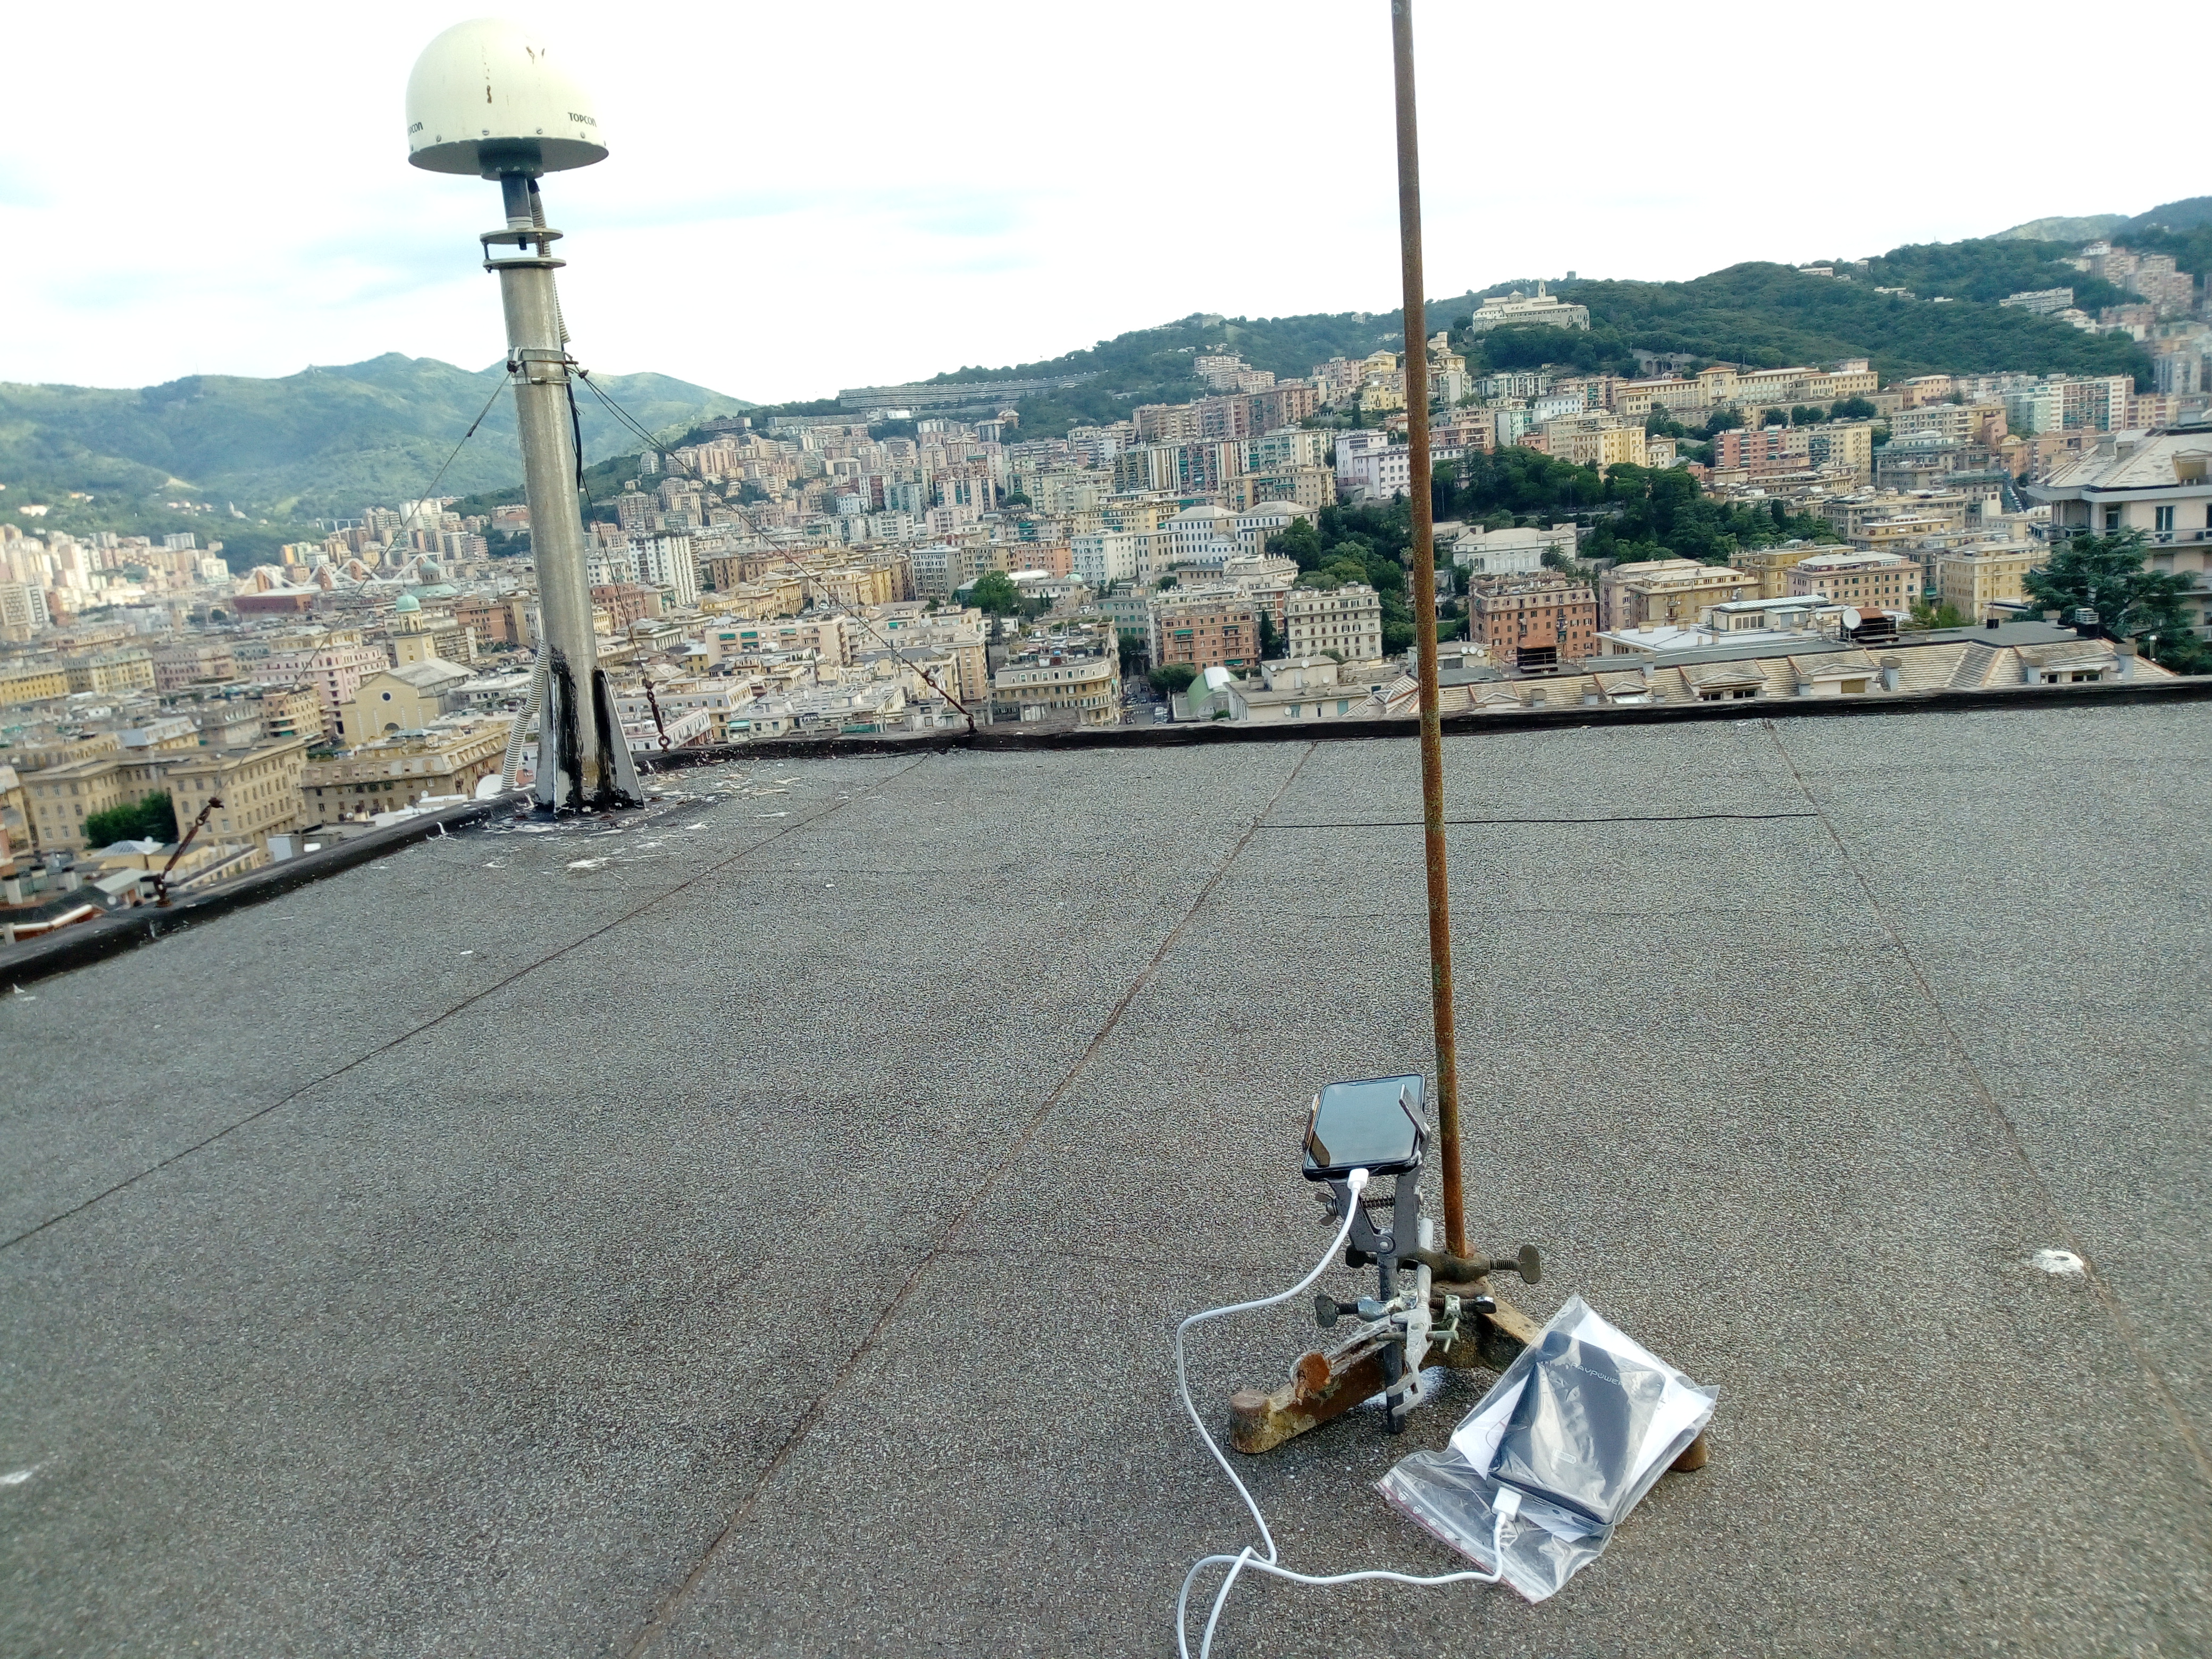
\includegraphics[scale=0.08]{fig/genu_test1.jpg} 
	\caption{test 1 setup}
	\label{FIG:test1} 
\end{figure}
The GENU receiver is part of the Ligurian RTK network. Therefore, its precise coordinates can be easily 
obtained obtained from it's monography. The precise coordinates for the smartphone receiver were obtained by 
means of a static positioning procedure based on the GENU receiver.
%
\subsection{Test 2:  Smartphone Orientations}
In a typical GNSS survey, the correct antenna position plays an important role in the quality of positioning. 
In the technical specifications of standard GNSS receivers, the user is often provided with the necessary information 
for a correct antenna positioning (i.e. mainly position of the phase centre, and orientation with respect to north). 
Smartphones, on the other hand, are not designed as classical GNSS receivers. In general, it is not always possible to get 
access on information about the antenna physical location inside the device.
For instance, the Xiaomi Mi8 smartphone equipped with Android 9 (updated in March 2022) used in our tests does
not give access to these information. Only since Android 11,  phase center offset coordinates and  
variation corrections have been added to the Raw Measurement API.
Test 2 aims at comparing different orientations of the device.
More specifically, five different static acquisition were then performed placing the smartphone on the same spot in  5 different orientations, as shown in Fig. \ref{FIG:test2_setup}.
\begin{figure}[H] 
	\centering
    \subfigure[]{\includegraphics[width=0.27\textwidth]{fig/test2_position1.jpg}} 
    \subfigure[]{\includegraphics[width=0.27\textwidth]{fig/test2_position2.jpg}} 
    \subfigure[]{\includegraphics[width=0.27\textwidth]{fig/test2_position3.jpg}} 
    \newline
    \subfigure[]{\includegraphics[width=0.27\textwidth]{fig/test2_position4.jpg}} 
    \subfigure[]{\includegraphics[width=0.27\textwidth]{fig/test2_position5.jpg}}    
    \caption{Test 2 acquisition with the smartphone in 5 different positions: (a) position 1 (b) position 2 (c) position 3 (d) position 4 (e) position 5}
    %\label{fig:foobar}
	\label{FIG:test2_setup} 
\end{figure}
As shown in the figure \ref{FIG:test2_setup}a, in position 1 the smartphone was oriented towards North and 
positioned horizontally, screen facing upwards. In the second position (figure \ref{FIG:test2_setup}b),
the smartphone was still facing north, but tilted at an angle of 45 degrees to the horizon, and screen 
facing upwards. In the third position (figure \ref{FIG:test2_setup}c) the smartphone is placed vertically with 
screen facing south. In the fourth position (figure \ref{FIG:test2_setup}d), the smartphone was oriented to  south and 
tilted 45 degrees to the horizon,  screen facing downwards. 
The last acquisition (Fig. \ref{FIG:test2_setup}e) was performed with the smartphone oriented to  south, 
placed horizontally, and screen facing downwards. 
The test was performed, in Manesseno (Genoa) on the 20\textsuperscript{th} of March 2020. 
Each acquisition lasted about half an hour in the following sequence:
\begin{itemize}
    \item position 1: from 15:20 to 15:50 UTC
    \item position 2: from 15:50 to 16:24 UTC
    \item position 3: from 16:32 to 16:57 UTC
    \item position 4: from 17:11 to 17:48 UTC
    \item position 5: from 17:48 to 18:21 UTC
\end{itemize}
\subsection{Test 3: Pedestrian Navigation}
Navigation is one of the main areas in which the GNSS receiver embedded into a smartphone is employed. 
Test 3 aims of making an assessment of the performance of the GNSS positioning from a smartphone in a typical 
scenarios such as  pedestrian navigation. 
More specifically, test 3 consists of a kinematic pedestrian acquisition involving two GNSS receivers: 
the Xiaomi Mi 8, and the Stonex S500, used as a term of comparison. The Stonex S500 is a single frequency (L1) 
and multi constellation (GPS, GLONASS, Galileo, and BeiDou) typically used for GIS (Geographic Information System) 
and RTK applications. 
The test was carried out on the 19\textsuperscript{th} of December 2021 in Genoa in Piazzale San Francesco d'Assisi, 
on a known path. The test path, shown in the figure \ref{FIG:test3_setup}a, was identified by determining the vertices of a 
square. In order to get the vertexes' coordinates with high precision, the four vertexes were surveyed in NRTK modality with 
the Stonex S70G, a geodetic level GNSS receiver, and exploiting the Ligurian NRTK network for getting the differential 
corrections. Once surveyed the vertexes were materialised using four targets. 
\begin{figure}[H] 
	\centering
    \subfigure[]{\includegraphics[width=0.48\textwidth]{fig/percorso_test3.jpg}} 
    \subfigure[]{\includegraphics[width=0.48\textwidth]{fig/test3_walk.jpg}} 
    \caption{(a) Path used for test 3 (b) Test 3 execution}
    %\label{fig:foobar}
	\label{FIG:test3_setup} 
\end{figure}
Test 3 started at vertex number 1 with a static acquisition of 2 minutes. 
After that a walk between the four vertexes was performed along the squared sides as depicted in Fig. \ref{FIG:test3_setup}a. 
Each side has been traversed in both directions (e.g. from vertex 1 to vertex 2 and from vertex 2 to vertex 1). 
The test ended at vertex 1 with a static acquisition of 2 minutes. Data from both the receivers were collected at 
1 Hz rate. During the test, the two receivers were held at a height of about 1 metre above the 
ground (see Fig. \ref{FIG:test3_setup}b).
\subsection{Test 4: Multipath Effect}
Multipath and other interferences are one of the main source of error in GNSS positioning in urban canyons, 
especially if mass market GNSS receivers are employed. Based on this consideration, test 4 aims in evaluating 
the impact of multipath  in smartphone positioning. Similarly to test 3, a second GNSS receiver is used for comparing 
positioning results. Test 4 consists then in static acquisition, in which, for a specific interval, the multipath effect 
was reproduced by placing a metal plate behind the receivers (see figure \ref{FIG:test4_setup}).

The receivers used in this test are the Xiaomi Mi 8, and the ublox ZED F9P coupled with the AN-MB-00 patch antenna. The ublox ZED F9P is a mass market multi-frequency (L1/L2) and multi-constellation (GPS, GLONASS, Galileo, and BeiDou) GNSS receiver.

\begin{figure}[H] 
	\centering
    \subfigure[]{\includegraphics[width=0.48\textwidth]{fig/test4_standard.jpg}} 
    \subfigure[]{\includegraphics[width=0.48\textwidth]{fig/test4_multipath.jpg}} 
    \caption{Test 4 acquisition under standard condition (a), and with multipath induced (b)}
   % \label{fig:foobar}
	\label{FIG:test4_setup} 
\end{figure}

Test 4 was performed in Villa Croce (Genoa) on the 10\textsuperscript{th} of March 2022. 
The two receivers were placed in a point whose coordinates were determined with high precision in NRTK modality using  the Stonex S70G receiver, and exploiting the Ligurian NRTK network for the differential corrections. The static acquisition started at 9:15 am UTC time and lasted 1 hour. From 9:45 to 10:00 the multipath effect was induced placing the metal plate behind the receivers (see Fig. \ref{FIG:test4_setup}). After 10:00 the plate was removed and the acquisition ended at 10:15. Data from both the receiver were 
collected at 1 Hz rate.

\section{Discussion}
In this section the test results together with the adopted processing strategies are explained in details. Before proceeding to the discussion of the results, it's useful to clarify the concepts of precision and accuracy of the measurements, which are two parameters used to evaluate the positioning performances. Accuracy refers to the degree of dispersion of individually measured data with respect to the mean value of the series to which they belong to. Precision, on the other hand, means the deviation between the measured data and the real or reference data (i.e. the precise coordinates of the point). Figure \ref{FIG:prec_vs_acc} illustrates the difference between precision and accuracy for a generic data set.

\begin{figure}[H] 
	\centering
	\includegraphics[scale=0.4]{fig/Precision-versus-accuracy.jpg} 
	\caption{Precision vs Accuracy}
	\label{FIG:prec_vs_acc} 
\end{figure}

Considerations on accuracy and precision of the solution can be made through the Standard Deviation (STD) and Root Mean Square (RMS) values. Given a set of elements STD and RMS can be defined as:

\begin{equation} 
	\begin{matrix} 
		STD= \sqrt{\frac{1}{N}\cdot \sum_{k=1}^N \left(x_{k}-\mu_{x}\right)^2 }\\ 
		RMS= \sqrt{\frac{1}{N}\cdot \sum_{k=1}^N \left(x_{k}-\tilde{x} \right)^2 }
		\end{matrix}
	\\
	\label{eq:std-rms}
\end{equation}
Where:
\begin{itemize}
\item $N$ is the total number of elements,
\item $x_{k}$ is a generic element belonging to the set,
\item $\mu_{x}$ is the mean value,
\item $\tilde{x}$ is a reference value for the elements (i.e., in this case, the precise coordinates of the point).
\end{itemize}

Given their definition, the STD can be considered an indicator of the precision, while the RMS can be considered an indicator of the accuracy.

\subsection{Processing Strategy}


All the processing exposed in this chapter were performed using the RTKLIB v 2.4.3 b34 software. In order to evaluate both accuracy and precision  accuracy the static tests processed as kinematic ones, i.e. obtaining as output a point cloud, with the coordinates computed epoch by epoch. Mainly two type of processing are performed: a Stand Alone positioning, which requires only the observable of the receiver in exam and a relative post processing which involves not only the observables of the receiver in exam but also the ones of a base station. This second processing is also called Post-Processed Kinematics (PPK). Unless otherwise specified the options used for processing are the following. 
The Ionosphere and Troposhere models used are the Klobuchar \cite{Klobuchar:1987} (which parameters are transmitted with the navigation message) and Saastamoinen \cite{Saastamoinen} respectively. For every tests only the broadcast ephemeris were considered and an elevation mask of \ang{15} is also set. 

Concerning the PPK elaborations the solution type combined was set. This options refers to the direction in time that the Kalman filter is run and its possible values are forward, backward and combined. Forward is the the only mode that can be used in real-time solutions (RTK). In this modality, the observation data is processed through the Kalman filter in the forward direction, i.e. starting with the beginning of the data and continuing through to the end. Backward mode is the opposite,  data is run through the filter starting with the end of the data and continuing to the beginning. In Combined mode, the filter is run both ways and the two results are combined into a single solution.


\subsection{Test 1}
In order to understand both the impact of the measurement noise in the positioning and quality of the positioning retrieved from the smartphone with respect to a geodetic receiver, two processing were computed: a Stand Alone, and a Post Processing with a common base receiver. In the Stand Alone processing only the pseudorange measurement are considered, and the two receiver are processed independently of each other. In order to make the results comparable, the constellation envolved in the processing were GPS and GLONASS, as GENU receiver was not able to track also Galileo and BeiDou as the smartphone. A cut off angle of \ang{15} was set for both the receivers. The chosen data rate for this elaboration is 1 Hz.
The results of the Stand Alone positioning for the two receivers are shown in Fig. \ref{FIG:test1_standalone}

\begin{figure}[H] 
	\centering
    \subfigure[]{\includegraphics[width=0.48\textwidth]{fig/test1/test1_stand_alone_groundtrck.jpg}} 
    \subfigure[]{\includegraphics[width=0.48\textwidth]{fig/test1/test1_stand_alone_timeserie.jpg}} 
    \caption{(a) Scatter plot of the positioning error for GENU (green) and Smartphone (red) receivers  (b) time series of the positioning error for GENU (green) and Smartphone (red) receivers}
    %\label{fig:foobar}
	\label{FIG:test1_standalone} 
\end{figure}

The values reported in Fig. \ref{FIG:test1_standalone} refers to the difference computed with respect to the precise coordinates for both the receivers. 
The statistics values, in terms of RMS and standard deviation, of such differences are reported in tab \ref{tab:test1_spp}.

\begin{table}[H]
	\centering
	\begin{tabular}{|c|p{1.5cm}|p{1.5cm}|p{1.5cm}|p{1.5cm}|p{1.5cm}|p{1.5cm}|}
	\hline
	\textbf{Receiver} & \textbf{RMS E [m]} & \textbf{RMS N [m]} &
	\textbf{RMS H [m]} &\textbf{STD E [m]}&\textbf{STD N [m]}&\textbf{STD H [m]}\\
    \hline
	GENU & 2.385 & 1.278& 3.729&0.965&0.884&3.441\\  
    \hline
	Smartphone & 4.207 & 5.723& 12.784&3.916&5.643&12.784\\ \hline
	\end{tabular} 
	\caption{Test 1, Stand Alone processing results}
	\label{tab:test1_spp}
\end{table}

With reference to the values in the Table \ref{tab:test1_spp} and Fig. \ref{FIG:test1_standalone} it is possible to state that the geodetic receiver and the smartphone presents a meter level accuracy, which is typical of this kind of positioning. The accuracy of the smartphone positioning however results definitely coarser than the one of the geodetic receiver. Also concerning the precision, the smartphone presents coarser results. Some outilers of the order of several tens of metres can also be detected between the smartphone positions. This behaviour can be explained by the poor quality of the smartphone observables compared to those of the geodetic receiver. An indicator of the quality of observables is the residual of the pseudorange measurements. The pseudorange residual is the difference between the value of the satellite-receiver range, computed a-posteriori (when the point coordinates are known) and the observed value. The residual plot for the two receivers in shown in Fig. \ref{FIG:test1_psdrgres}

\begin{figure}[H] 
	\centering
    \subfigure[]{\includegraphics[width=0.48\textwidth]{fig/test1/test1_psdrg_residual_xiaomi.jpg}} 
    \subfigure[]{\includegraphics[width=0.48\textwidth]{fig/test1/test1_psdrg_residual_genu.jpg}} 
    \caption{(a) Residual pseudorange plot for Smartphone receiver (b) Residual pseudorange plot for GENU receiver}
   % \label{fig:foobar}
	\label{FIG:test1_psdrgres} 
\end{figure}

It is possible to state form Fig. \ref{FIG:test1_psdrgres} that pseudorange residuals from smartphone are definitely noisier than the ones from the GENU receiver. This can be explained by the different quality of the antennas which the two receivers mounts: GENU receiver in fact has a choke ring antenna, which is used for precise positioning purposes while the smartphone has an integrated antenna not specifically designed for GNSS positioning.    

Test 1 receivers have been also post processed with a common reference station. The base receiver chosen is GENO, a GNSS receiver of the RDN (Rete Dinamica Nazionale)\footnote{\url{https://www.igmi.org/it/direzione-geodetica}} located approximately 3 km away from the test field.

The obtained results are shown in figure \ref{FIG:test1_pp}

\begin{figure}[H] 
	\centering
    \subfigure[]{\includegraphics[width=0.48\textwidth]{fig/test1/test1_pp_groundtrck.jpg}} 
    \subfigure[]{\includegraphics[width=0.48\textwidth]{fig/test1/test1_pp_timeserie.jpg}} 
    \caption{(a) Scatter plot of the positioning error for GENU (green) and Smartphone (red) receivers  (b) time series of the positioning error for GENU (green) and Smartphone (red) receivers}
    %\label{fig:foobar}
	\label{FIG:test1_pp} 
\end{figure}

The statistics values, in terms of RMS and standard deviation with respect to the precise coordinates of the receivers, are reported in Table \ref{tab:test1_pp}

\begin{table}[H]
	\centering
		\begin{tabular}{|c|p{1.5cm}|p{1.5cm}|p{1.5cm}|p{1.5cm}|p{1.5cm}|p{1.5cm}|}
	\hline
	\textbf{Receiver} & \textbf{RMS E [m]} & \textbf{RMS N [m]} &
	\textbf{RMS H [m]} &\textbf{STD E [m]}&\textbf{STD N [m]}&\textbf{STD H [m]}\\
	\hline
	GENU & 0.004 & 0.001 & 0.005&0.003&0.0004&0.003\\  
    \hline
	Smartphone & 0.576 & 0.242& 0.333&0.167&0.152&0.158\\ \hline
	\end{tabular} 
	\caption{Test 1, Post processing results}
	\label{tab:test1_pp}
\end{table}

The GENU receiver has an RMS in the order of millimetres for all the components. The standard deviations in East, North and Height components are also in the millimetre range. Those are expected results for a geodetic GNSS receivers. The smartphone receiver in the other hand presents coarser results with respect to the geodetic one. The RMS are in the order of tens of centimeters with a maximum of 58 cm in the East. Also the standard deviations is in the order of tens of centimeters with a maximum in the Height component equal to 17 cm.      
The two positioning can be also compared in terms of percentage of fixing solutions obtained. The smartphone positioning only have 1 fixing solution (i.e. 0.1\%) while GENU receiver have 127 fixing solutions (i.e. 15.4\%). Furthermore the only fixing solution of the smartphone (blue point in Fig. \ref{FIG:test1_pp}a  can be considered an outlier as its error values are not coherent with the rest of the obtained errors. It's error components for East, North and Height components in fact are -1.306 m, 3.899 m and 2.753 m respectively with respect to the precise coordinates of the point. Considering that for fixed solutions the expected errors are in the order of few centimeters, this point can be also considered a false fixed solution.   

\subsection{Test 2}
Similarly to test 1, also for test 2 two processing were computed in order to evaluate whether the smartphone orientation influences the positioning results. The first one is a Stand Alone processing and the second one is a PPK processing with GENU receiver. The baseline between the smartphone receiver and the GENU base, in this case is about 10 km. Considering the length of the baseline and the low quality of smartphone hardware in this case it was not possible to determine the precise coordinates of the smartphone. Considering that and than only consideration concerning the precision and not the accuracy can be carried out for this case study. Nevertheless it interesting to report this case also to show the behaviour of relative positioning from smartphone considering long baselines.

The result for the Stand Alone processing are exposed in Fig. \ref{FIG:test2_sa_scatter}:

\begin{figure}[H] 
	\centering
    \subfigure[]{\includegraphics[width=0.3\textwidth]{fig/test2/test2_p1_sa.jpg}} 
    \subfigure[]{\includegraphics[width=0.3\textwidth]{fig/test2/test2_p2_sa.jpg}} 
    \subfigure[]{\includegraphics[width=0.3\textwidth]{fig/test2/test2_p3_sa.jpg}} 
    \newline
    \subfigure[]{\includegraphics[width=0.3\textwidth]{fig/test2/test2_p4_sa.jpg}} 
    \subfigure[]{\includegraphics[width=0.3\textwidth]{fig/test2/test2_p5_sa.jpg}}    
    \caption{Scatter plot of the positioning error for test 2 in Stand Alone modality: (a) position 1 (b) position 2 (c) position 3 (d) position 4 (e) position 5}
   % \label{fig:foobar}
	\label{FIG:test2_sa_scatter} 
\end{figure}

Table \ref{tab:test2_sa} shows the standard deviation for the position errors obtained:

\begin{table}[H]
	\centering
	\begin{tabular}{|c|c|c|c|}
	\hline
	\textbf{Position} &\textbf{STD E [m]}&\textbf{STD N [m]}&\textbf{STD H [m]}\\
    \hline
	 1 & 3.352 & 4.833  & 10.286\\  
    \hline
     2 & 3.040 & 5.455  & 7.391\\  
    \hline
     3 & 2.982 & 5.474  & 6.265\\  
    \hline
     4 & 3.572 & 3.857  & 14.188\\  
    \hline
     5 & 3.276 & 4.655  & 11.436\\  
    \hline
	\end{tabular} 
	\caption{Test 1, Post processing results}
	\label{tab:test2_sa}
\end{table}

The standard deviation values derived from the five different positions are in agreement with each other and settle at values of about 3 m in the East component, about 5 m in the North component and about 10 m in the Height component. These values are also of the same order of magnitude as those obtained for the Stand Alone positioning of test 1 (cfr Table \ref{tab:test1_spp}). Therefore, there does not seem to be one position that clearly prevails over another in terms of precision in smartphone Stand Alone positioning.

As previously stated nothing can be said about the positioning accuracy, as it was not possible to determine the precise coordinates of the smartphone.

The results of the PPK processing with GENU base are exposed in Fig. \ref{FIG:test2_pp_scatter} 

\begin{figure}[H] 
	\centering
    \subfigure[]{\includegraphics[width=0.3\textwidth]{fig/test2/test2_p1_pp.jpg}} 
    \subfigure[]{\includegraphics[width=0.3\textwidth]{fig/test2/test2_p2_pp.jpg}} 
    \subfigure[]{\includegraphics[width=0.3\textwidth]{fig/test2/test2_p3_pp.jpg}} 
    \newline
    \subfigure[]{\includegraphics[width=0.3\textwidth]{fig/test2/test2_p4_pp.jpg}} 
    \subfigure[]{\includegraphics[width=0.3\textwidth]{fig/test2/test2_p5_pp.jpg}}    
    \caption{Scatter plot of the positioning error for test 2 in Post Processing: (a) position 1 (b) position 2 (c) position 3 (d) position 4 (e) position 5}
   % \label{fig:foobar}
	\label{FIG:test2_pp_scatter} 
\end{figure}

Table \ref{tab:test2_pp_fixflt} shows the standard deviation for the position errors obtained:

\begin{table}[H]
	\centering
	\begin{tabular}{|c|c|c|c|}
	\hline
	\textbf{Position} &\textbf{STD E [m]}&\textbf{STD N [m]}&\textbf{STD H [m]}\\
    \hline
	 1 & 4.017 & 6.061  & 9.282\\  
    \hline
     2 & 7.692 & 2.373  & 3.896\\  
    \hline
     3 & 9.854 & 4.217  & 9.365\\  
    \hline
     4 & 4.834 & 5.732   & 7.379 \\  
    \hline
     5 & 5.168 &  4.316& 9.925\\  
    \hline
	\end{tabular} 
	\caption{Test 1, Post processing results}
	\label{tab:test2_pp_fixflt}
\end{table}

From the graphs shown in the Fig. \ref{FIG:test2_pp_scatter} and the values in the Table \ref{tab:test2_pp_fixflt}, it can be state that PPK from smartphones on long baselines has precision errors in the order of meters, while sub metric values are attended for this type of techniques. It can be also said that all the fixed solution obtained are false fixing solutions as their error values are clearly not coherent with the rest of the obtained errors. 
Factors explaining this behaviour are the poor quality of GNSS data from smartphones and the length of the baseline. For the rest of the tests carried out in this work only shorter baselines ($<$ 1 Km) are then considered.
Also considering the post processing approach, it seems that none of the positions tested shows better results if compared to the others. Based on this, for the rest of the tests carried out in this work, no further attention will be paid to the orientation of the smartphone.


\subsection{Test 3}


The performance of the smartphone GNSS receiver in a kinematic contest can be analysed at two different levels: preprocessing level and positioning level. In both cases to better understand its performance, the data coming from the smartphone (Xiaomi Mi 8) are compared with the ones coming from the Stonex S500 receiver, which is considered as a benchmark.

Concerning the preprocessing level the quality of the incoming signal for the two receiver is compared. A good indicator of the incoming signal quality is the Signal to Noise Ratio (SNR), which is measure of the strength of the desired signal relative to background noise. SNR expressed in DB-Hz presents high values for a good incoming signal, while low values for a bad signal. The SNR values for the two receivers used in test 3 are shown in Fig. \ref{FIG:test3_snr}.

\begin{figure}[H] 
	\centering
    \subfigure[]{\includegraphics[width=0.48\textwidth]{fig/test3/test3_snr_xiaomi.jpg}} 
    \subfigure[]{\includegraphics[width=0.48\textwidth]{fig/test3/test3_snr_s500.jpg}} 
    \caption{SNR for Xiaomi Mi 8 receiver (a) and for Stonex S500 receiver (b) }
    %\label{fig:foobar}
	\label{FIG:test3_snr} 
\end{figure}

Figure \ref{FIG:test3_snr} shows that the Stonex S500 receiver has a much better SNR than the Xiaomi Mi 8 receiver. In fact an average difference of about 10 DB-Hz between the two receivers is observed. From the SNR trend it's also possible to recognise the static and kinematic parts of the survey. The kinematic part, highlighted in the green dashed box, in fact presents a noisier SNR trend than the static parts located at the beginning at ad the end of the test.

It's also interesting to notice that number of satellites acquired by the two receivers (Fig. \ref{FIG:test3_nsat}).

\begin{figure}[H] 
	\centering
    \subfigure[]{\includegraphics[width=0.48\textwidth]{fig/test3/test3_nsat_xiaomi.jpg}} 
    \subfigure[]{\includegraphics[width=0.48\textwidth]{fig/test3/test3_nsat_s500.jpg}} 
    \caption{Number of satellite observed by Xiaomi Mi 8 receiver (a) and Stonex S500 receiver (b) }
   % \label{fig:foobar}
	\label{FIG:test3_nsat} 
\end{figure}

The number of satellites observed by the Xiaomi Mi 8 is greater than that of the Stonex S500, but much more variable over time. In fact, the Xiaomi Mi 8 receiver also acquires very noisy satellites (SNR $<$ 25 DB-Hz) for short periods of time, which are ignored by the Stonex S500. However, acquiring a larger number of satellites is not always advantageous for positioning purposes, especially if the acquired signals are very noisy. 


Concerning the positioning part, both the receiver were post processed with a common GNSS permanent station located about 200 m away from the test field. This GNSS permanent station, hereafter called LIGE, was designed and realized in the ambit of this thesis work (see par \ref{par:lige}). LIGE permanent station is equipped with the low cost GNSS receiver Ublox ZED F9P coupled with the Hemisphere A45 antenna. 
For this case study the solution type "forward" is set in order to simulate a real time condition. 

The positioning solutions obtained are shown in Fig. \ref{FIG:test3_pp}.

\begin{figure}[H] 
	\centering
    \subfigure[]{\includegraphics[width=0.48\textwidth]{fig/test3/test3_pp_scatter.jpg}} 
    \subfigure[]{\includegraphics[width=0.48\textwidth]{fig/test3/test3_pp_timeserie.jpg}} 
    \caption{(a) Scatter plot of the positioning error for Xiaomi Mi8 and Stonex S500  (b) time series of the positioning error for Xiaomi Mi8 and Stonex S500}
   % \label{fig:foobar}
	\label{FIG:test3_pp} 
\end{figure}

Considering that the first two minutes and the last two minutes of the survey were carried out statically at vertex P1 (see Fig. \ref{FIG:test3_setup}), it is possible to make preliminary considerations on the accuracy of the positioning obtained by comparing the deviation of the positions obtained in the first two minutes and the last two minutes with respect to the precise coordinates of the vertex.
The Xiaomi Mi8 receiver presents and RMS of 1.066 m, 2.849 m and 5.670m for East, North and Height components respectively while the Stonex S500 has 0.598 m, 0.498 and 2.318 m for East, North and Height components respectively. The Stonex S500 receiver solution is therefore more accurate, especially when considering the North and Altitude components.


The two solutions can be compared also in terms of number of computed positions and percentage of fix and float solutions (see Table \ref{tab:test3_pp_quality}).

\begin{table}[H]
	\centering
	\begin{tabular}{|c|c|c|c|}
	\hline
	\textbf{Receiver} &\textbf{Number of solutions}&\textbf{Fixed solutions}&\textbf{Float solutions}\\
    \hline
	 Xiaomi Mi 8 & 595 & 19 (3,2\%) & 576 (96.8\%)\\  
    \hline
     Stonex S500 & 617 & 47 (7,6\%) & 570 (92.4\%)\\  
    \hline
	\end{tabular} 
	\caption{Test 3, Solution quality}
	\label{tab:test3_pp_quality}
\end{table}

The Xiaomi Mi 8 receiver presents fewer solutions than the Stonex S500. The poor quality of the GNSS measurement from the smartphone prevents the computation of the positioning for some epochs. Furthermore the Xiaomi Mi 8 solution, coherently with other results obtained from the previous tests presents some outliers and false fixing solutions.


\subsection{Test 4}
Similarly to test 3, also for this case the performance of the Xiaomi Mi8 receiver are compared to the ones of the other device involved, the Ublox ZED F9P in two different levels: preprocessing and positioning level. Once again in the preprocessing level the two receivers are compared in terms of quality of the incoming signal. For this purpose the SNR trend for the two receivers is shown in Fig. \ref{FIG:test4_snr}.
\begin{figure}[H] 
	\centering
    \subfigure[]{\includegraphics[width=0.48\textwidth]{fig/test4/test4_snr_xiaomi.jpg}} 
    \subfigure[]{\includegraphics[width=0.48\textwidth]{fig/test4/test4_snr_ublox.jpg}} 
    \caption{SNR for Xiaomi Mi 8 receiver (a) and for Ublox ZED F9P receiver (b) }
  %  \label{fig:foobar}
	\label{FIG:test4_snr} 
\end{figure}

Concerning the SNR comparison, the results obtained for test 3 are confirmed also for this case study. The Xiaomi Mi 8 on average presents lower SNR values with respect to the Ublox ZED F9P. This means that, due to the poor quality of the smartphone's hardware, the signals acquired by the Xiaomi Mi 8 receiver are much noisier. From the SNR trend of the two receivers it's evident the period in which the multipath effect was induced with the metal plate, i.e. from 9:45 a.m. to 10:00 a.m. UTC (green boxes in Fig. \ref{FIG:test4_snr}). In this time interval, as expected, the signals acquired is degraded.This results in a general lowering of SNR values, and a significantly noisier trend. 


Concerning the positioning part, both the receiver were post processed with a the LIGE permanent station which is about 0.2 km away from the test field. Similarly to test 3 also for this case study the solution type chosen is forward. Figure \ref{FIG:test4_pp} shows the obtained positioning results in terms of errors with respect to the precise coordinates of the point.

\begin{figure}[H] 
	\centering
    \subfigure[]{\includegraphics[width=0.48\textwidth]{fig/test4/test4_pp_scatter.jpg}} 
    \subfigure[]{\includegraphics[width=0.48\textwidth]{fig/test4/test4_pp_timeserie.jpg}} 
    \caption{(a) Scatter plot of the positioning error for Xiaomi Mi8 and Ubox ZED F9P  (b) time series of the positioning error for Xiaomi Mi8 and Ubox ZED F9P}
    %\label{fig:foobar}
	\label{FIG:test4_pp} 
\end{figure}

The statistics values, in terms of RMS and standard deviation with respect to the precise coordinates of the receivers, are reported in Table \ref{tab:test4_pp}.

\begin{table}[H]
	\centering
	\begin{tabular}{|c|p{1.5cm}|p{1.5cm}|p{1.5cm}|p{1.5cm}|p{1.5cm}|p{1.5cm}|}
	\hline
	\textbf{Receiver} & \textbf{RMS E [m]} & \textbf{RMS N [m]} &
	\textbf{RMS H [m]} &\textbf{STD E [m]}&\textbf{STD N [m]}&\textbf{STD H [m]}\\
    \hline
	Xiaomi Mi8 & 0.499 &0.549 &0.556  &0.133 & 0.151&0.411\\  
    \hline
	Ublox ZED F9P & 0.021 & 0.043 & 0.020&0.179&0.017&0.018\\ \hline
	\end{tabular} 
	\caption{Test 4, Post processing results}
	\label{tab:test4_pp}
\end{table}

In this case study the solution for the Xiaomi Mi8 receiver has a convergence time of about 5 minutes. After this time interval the standard deviation of the solution are 0.051 m, 0.08 m, 0.093 m for East, North and Height components respectively.The solutions then presents a centimeter level accuracy, nevertheless the Ublox ZED F9P solution result more accurate. After the convergence time the Xiaomi Mi8 solution has average deviations from the precise point coordinates of -0.460m, -0.549m and 0.390m for East, North and Height components respectively. It can be state that the solution presents a decimeter precision level, but once again the Ublox ZED F9P solution results more precise.

Similarly to the previous tests the two solution can be compared in term of number of solutions and percentage of fix solution obtained. Coherently to the results already obtained for the other case studies, the Xiaomi Mi8 has a lower number of solutions (3473 against 3501) and a lower percentage of fixed solutions (2.4\% against 81.3\%).

For this case study it's also interesting to anal the solution in the time interval in which the multipath was induced, i.e. between the 9:45 and the 10:00 UTC. For the Ublox ZED F9P the solution results particularly degraded (see Fig. \ref{FIG:test4_pp}b), and almost the totality of the float solutions obtained for this receiver is in this time interval. Concerning the Xiaomi receiver the solution doesn't seem particularly degraded in this time interval with respect of the entire test period, nevertheless in this interval some false fixed solution can be observed. 

In this chapter an assessment of the quality of the GNSS position from a smartphone receiver is performed. For this purpose many tests were performed under different boundary condition and using different processing techniques, in this chapter the 4 most significant tests were reported and commented. Summarising the obtained results it's possible to state that on average the quality of the satellite signal received for smartphone receiver is definitely lower with respect to both geodetic GNSS receiver (e.g. GENU receiver in test one), but also to mass market GNSS receiver (e.g. Ublox ZED F9P in test 4). This is due to the low quality of the smartphone hardware, in particular of the antenna which is not designed for GNSS positioning. Concerning Stand Alone positioning typical accuracy and precision obtained from a smartphone are in the order of few meters. Concerning post processing relative positioning, the accuracy and precision are in the order of decimeters in both static and kinematic situations. It can be also state that in post processing approach the phase ambiguity can be hardly fixed with smartphone's observables. Furthermore the fix solution obtained are often false fixed. These false fixed solutions together with other outliers definitely compromise the robustness of the GNSS positioning by smartphone. 